\documentclass[10pt]{beamer}

\usetheme{metropolis}
\usepackage{appendixnumberbeamer}

\usepackage{booktabs}
\usepackage[scale=2]{ccicons}

\usepackage{pgfplots}
\usepgfplotslibrary{dateplot}

\usepackage{xspace}
\newcommand{\MDL}{\textbf{\textsc{mdl}}\xspace}

\usepackage{graphicx}
\usepackage{tikz-cd}

\newcommand{\Cat}[1]{\ensuremath{\underline{\mathbf{#1}}}}
\newcommand{\Obj}[1]{\ensuremath{\mathrm{Obj}(\Cat{#1})}}
\newcommand{\Hom}[3]{\ensuremath{\mathrm{Hom}_{\Cat{#1}}(#2,#3)}}
\newcommand{\Domain}[1]{\ensuremath{\mathbf{Dom}(#1)}}
\newcommand{\Codomain}[1]{\ensuremath{\mathbf{Cod}(#1)}}
\newcommand{\CompCat}[1]{\Cat{\overline{#1}}}
\newcommand{\Comm}[1]{\mathrm{Kom}_{\Cat{#1}}}
\newcommand{\Com}[3]{#3^{#2}}
\newcommand{\SCat}[1]{\Cat{Symms(#1)}}
\newcommand{\FSCat}[1]{\Cat{FSymm(#1)}}
\newcommand{\FkCat}[1]{\Cat{FkSymm(#1)}}
\newcommand{\PkCat}[1]{\Cat{PkSymm(#1)}}
\newcommand{\IrPaths}[1]{\Cat{IrPaths(#1)}}
\newcommand{\FProj}[2]{\ensuremath{W_{\Cat{#1,#2}}}}
\newcommand{\FuncIm}[1]{\mathrm{Im}(#1)}
\newcommand{\term}[1]{\emph{#1}}
\newcommand{\strong}[1]{\textbf{#1}}

%% BEGIN Conal Elliott paper macros
\newcommand{\program}[1]{\texttt{#1}}
\newcommand{\id}{\mathtt{id}}
\newcommand{\apply}{\mathtt{apply}}
\newcommand{\curry}{\mathtt{curry}}
\newcommand{\uncurry}{\mathtt{uncurry}}
\newcommand{\exl}{\mathtt{exl}}
\newcommand{\exr}{\mathtt{exr}}
\newcommand{\termin}{\mathtt{1}}
\newcommand{\termarr}{\mathtt{it}}
\newcommand{\unitarrow}{\ensuremath{\mathtt{unitarrow}}}
\newcommand{\lamf}[2]{\ensuremath{\lambda\, #1 \mapsto #2}}
\newcommand{\lamtoccc}[1]{\ensuremath{\frak{K}(#1)}}
\newcommand{\delprod}[2]{\ensuremath{#1\,\Delta\,#2}}
\newcommand{\const}{\ensuremath{\mathtt{const}}}
\newcommand{\constFun}{\ensuremath{\mathtt{constFun}}}
%% END Conal Elliott paper macros

\newcommand{\eqnlabel}[1]{\label{eq:#1}}
\newcommand{\eqnref}[1]{(\ref{eq:#1})}
\newcommand{\deflabel}[1]{\label{def:#1}}
\newcommand{\defref}[1]{definition \ref{def:#1}}
\newcommand{\thlabel}[1]{\label{th:#1}}
\newcommand{\thref}[1]{theorem \ref{th:#1}}

% \newcommand{\pullback}{\arrow[d,]}
% \newcommand{\pushout}{\arrow[d,\text{\pigpenfont J}]}

% \newtheorem{threm}{Theorem}[section]
% \newtheorem{lemma}[threm]{Lemma}
\theoremstyle{definition}
% \newtheorem{corollary}[theorem]{Corollary}
% \newtheorem{definition}[theorem]{Definition}
% \newtheorem{example}[theorem]{Example}
\newtheorem{xca}[theorem]{Exercise}

\theoremstyle{remark}
\newtheorem{remark}[theorem]{Remark}

\numberwithin{equation}{section}

%    Absolute value notation
\newcommand{\abs}[1]{\lvert#1\rvert}

%    Blank box placeholder for figures (to avoid requiring any
%    particular graphics capabilities for printing this document).
\newcommand{\blankbox}[2]{%
  \parbox{\columnwidth}{\centering
%    Set fboxsep to 0 so that the actual size of the box will match the
%    given measurements more closely.
    \setlength{\fboxsep}{0pt}%
    \fbox{\raisebox{0pt}[#2]{\hspace{#1}}}%
  }%
}


\title{Compiling to Categories}
\subtitle{mathematically-principled program transformation}
% \subtitle{Our attempt to explain what Conal Elliott is up to}
\date{\today}
\author{T. Mark Ellison and Siva Kalyan}
\institute{Australian National University}
% \titlegraphic{\hfill\includegraphics[height=1.5cm]{logo.pdf}}

\usepackage{listings}
\usepackage{color}
\definecolor{identifierColor}{rgb}{0.65,0.16,0.16}
\lstset{
  frame=none,
  xleftmargin=2pt,
  stepnumber=1,
  numbers=left,
  numbersep=5pt,
  numberstyle=\ttfamily\tiny\color[gray]{0.3},
  belowcaptionskip=\bigskipamount,
  captionpos=b,
  escapeinside={*'}{'*},
  language=haskell,
  tabsize=2,
  emphstyle={\bf},
  commentstyle=\it\color{brown},
  stringstyle=\mdseries\rmfamily\color{green},
  showspaces=false,
  keywordstyle=\bfseries\rmfamily\color{red},
  columns=flexible,
  basicstyle=\small\sffamily\color{blue},
  showstringspaces=false,
  morecomment=[l]\%,
}

\begin{document}

%% SEE https://wiki.haskell.org/wikiupload/8/85/TMR-Issue13.pdf#page=73

\maketitle

\begin{frame}{Table of contents}
  \setbeamertemplate{section in toc}[sections numbered]
  \tableofcontents[hideallsubsections]
\end{frame}


\begin{frame}[fragile]
  \frametitle{Haskell and Category Theory}

  \begin{tabular}{lr}
    \toprule
    Haskell & Category Theory \\
    \midrule
    \textbf{Category} & \textbf{Category} \\
    \textbf{Type} & \textbf{Object} \\
    \textbf{Function} & \textbf{Morphism} \\
    \textbf{\Cat{Hask}} & \textbf{\Cat{Set}} \\
    \textbf{...} & \textbf{Terminal Objects} \\
    \textbf{Value} & \textbf{Global Element} \\
    \textbf{Tuple} & \textbf{Product} \\
    \textbf{Currying, Function Application} & \textbf{Cartesian Closure} \\
    \textbf{Type Constructor, Functor} & \textbf{Functor} \\
    \textbf{...} & \textbf{Natural Transformation} \\
    \textbf{Applicative} & \textbf{...} \\
    \textbf{...} & \textbf{Adjoint Functor Pair} \\
    \textbf{Monad} & \textbf{Monad} \\
    \bottomrule
  \end{tabular}

\end{frame}

\section{Categories}

\subsection{Basics}

\begin{frame}[fragile]
  \frametitle{Categories}

  A \emph{category} $\Cat{C}$ consists of
  \begin{enumerate}
  \item a class $\Obj{C}$ of \emph{objects}, and
  \item for each pair of objects $A,B \in \Obj{C}$, a set $\Hom{C}{A}{B}$
    of \emph{arrows} (or \emph{morphisms}) from $A$ to $B$, known as
    a \emph{hom-set}.
  \end{enumerate}\vspace{-1.5\baselineskip}

  \[
    \begin{tikzcd}
      A \arrow[shift left=2]{r}{\Hom{C}{A}{B}} \arrow{r} \arrow[shift right=2]{r} & B
    \end{tikzcd}
  \]

  Many familiar parts of Haskell form a category \Cat{Hask}:
  objects are \emph{types} (\lstinline{Int}, \lstinline{Char}, etc.),
  and arrows are \emph{functions} between types (e.g.\ \lstinline{ord :: Int -> Char}).
\end{frame}

\begin{frame}[fragile]
  \frametitle{Category Laws}
  In a category $\Cat{C}$:
  \begin{enumerate}
  \item Given arrows $f\colon A \rightarrow B$ and $g\colon B \rightarrow C$ in
    $\Cat{C}$, the \emph{composition} $g \circ f \colon A \rightarrow C$ (= \lstinline{g.f}) is also in
    $\Cat{C}$.
  \item Given arrows $f\colon A \rightarrow B$, $g\colon B \rightarrow C$ and $h\colon C \rightarrow D$, $(h \circ
    g) \circ f = h \circ (g \circ f) = h \circ g \circ f$:\vspace{-0.5\baselineskip}
    \[
      \begin{tikzcd}
        A \arrow{r}{f} \arrow[sloped,near end,swap,dashed]{dr}{g \circ f} \arrow[bend
        right=60,sloped,swap,loosely dashed]{drr}{h \circ g \circ f} \arrow[bend
        left=60,sloped,loosely dashed]{drr}{h
          \circ g \circ f} & B \arrow{d}{g}
        \arrow[sloped,near start,dashed]{dr}{h \circ g} & \\
          & C \arrow[swap]{r}{h} & D
      \end{tikzcd}\rlap{.}
    \]
  \item Every object $A \in \Obj{C}$ is associated with an \emph{identity arrow}
    $1_A \colon A \rightarrow A$ (= \lstinline{id}). Given any arrow $f\colon A \rightarrow B$, we have
    \[
      \begin{tikzcd}
        A \arrow[densely dotted]{r}{1_A} \arrow[bend right=30,swap]{rr}{f} & A
        \arrow["f" description]{r}
        \arrow[bend left=30]{rr}{f} & B \arrow[swap,densely dotted]{r}{1_B} & B
      \end{tikzcd}\rlap{.}
    \]
  \end{enumerate}
\end{frame}

\begin{frame}[fragile]
  \frametitle{Examples}

  \begin{center}
    \begin{tabular}{r l l l l}\toprule
    & $\Cat{Set}$ & $\Cat{Hask}$ & $\Cat{POrd}$ & $\Cat{Cat}$ \\\midrule
    \textbf{Objects} & sets & types & items & small cats \\
    \textbf{Morphisms} & functions & functions & $a \leq b$ & functors \\
    \textbf{Composition} & $f \circ g$ & \lstinline!f.g! & transitivity & $F \circ G$ \\
    \textbf{Identity} & $1_A$ & {\lstinline!id!} & $a = a$ & $1_{\Cat{C}}$ \\\bottomrule
  \end{tabular}
  \end{center}

  Not everything in Haskell can be in $\Cat{Hask}$ if we want it to be a category. Every type in the language contains a \lstinline{Bottom} ($\bot$) or \lstinline{undefined} value, but these 'values' cause mayhem with the category laws (in particular the \textbf{Identity} constraint). So when we talk about \Cat{Hask} we'll be talking about vanilla \Cat{Hask} without these abnormal values.
  {\small Haskell wiki page on \Cat{Hask}}
\end{frame}

\begin{frame}[fragile]{Category Theory: Terminal Objects}

  A \emph{terminal object} is a type $1$ (a.k.a.\ $T$) in $\Obj{C}$, such that there is only a single mapping from any other type $A$ onto that type:

  \[
    \forall A\in \Obj{C}, \left| \Hom{C}{A}{1} \right| = 1.
  \]

  \[
    \begin{tikzcd}[row sep=tiny]
      A \arrow[near start]{dr}{\exists!} & \\
      B \arrow["\exists!" description]{r} & 1\\
      C \arrow[swap,near start]{ur}{\exists!} & 
    \end{tikzcd}
  \]
  
  % Terminal objects in categories:
  % \begin{description}
  %   \item[\Cat{Set}] the singleton set
  %   \item[\Cat{Grp}] the singleton group
  %   \item[\Cat{Top}] the singleton topological space
  %   \item[\Cat{1\downarrow Set}] the singleton pointed set
  %   \item[\Cat{POrd}] the maximum element (if there is one)
  % \end{description}

  In \Cat{Hask}:
  \begin{lstlisting}[frame=single]
    () -- the type corresponding to 1, containing only itself
    terminalMap :: t -> ()
    terminalMap _ = ()
  \end{lstlisting}

\end{frame}

\begin{frame}[fragile,fragile]{Global Elements}
  %% See answer 4 here: http://stackoverflow.com/questions/17380379/where-do-values-fit-in-category-of-hask
  A \emph{global element} of an object $A$ in category $\Cat{C}$ with terminal object $1$ is an arrow $a : 1 \rightarrow A$.\vspace{-\baselineskip}
  
  \[
  \begin{tikzcd}
    1 \arrow{r}{a} & A
  \end{tikzcd}
  \]

  In \Cat{Hask}, if we have a value \lstinline{v} in some type \lstinline{a}, we
  can upgrade it to the global element by use of \lstinline{const v}.

  \begin{lstlisting}[frame=single]
    const :: a -> b -> a -- but for our purposes, choose b = ()
    const v = \ _ -> v
  \end{lstlisting}

\end{frame}

\begin{frame}[fragile]
  \frametitle{Examples}

  \begin{center}
    \begin{tabular}{r l l l l}\toprule
    & $\Cat{Set}$ & $\Cat{Hask}$ & $\Cat{POrd}$ & $\Cat{Cat}$ \\\midrule
    \textbf{Objects} & sets & types & items & small cats \\
    \textbf{Morphisms} & functions & functions & $a \leq b$ & functors \\
    \textbf{Composition} & $f \circ g$ & \lstinline!f.g! & transitivity & $F \circ G$ \\
    \textbf{Identity} & $1_A$ & {\lstinline!id!} & $a = a$ & $1_{\Cat{C}}$ \\
%%    \textbf{Initial obj\rlap{.}} & $\emptyset$ & \texttt{Void} & lwr bnd & $\Cat{0}$ \\
      \textbf{Terminal obj\rlap{.}} & $\{*\}$ & \lstinline!()! & upper bound & $\Cat{1}$ \\\bottomrule
  \end{tabular}
  \end{center}
  
\end{frame}

\begin{frame}[fragile]{Products}

  Given objects $A$, $B$ in $\Cat{C}$ there may be a \emph{(pairwise) product}
  $A\sqcap B \in \Obj{C}$ and \emph{projection arrows} $\pi_A \colon A \sqcap B \rightarrow A$ and
  $\pi_B \colon A \sqcap B \rightarrow B$ such that for any object $X$ in the same category and arrows
  $a \colon X \rightarrow  A$ and $b \colon X \rightarrow B$
  there is a \emph{unique} arrow $x : X \rightarrow A \sqcap B$ such that $a = \pi_A \circ x$ and $b = \pi_B \circ x$:

  \[
  \begin{tikzcd}
    A & A\sqcap B \arrow[swap]{l}{\pi_{A}} \arrow{r}{\pi_{B}} & B \\
    & X \arrow[dotted]{u}{\exists! x} \arrow{ul}{a} \arrow[swap]{ur}{b} & 
  \end{tikzcd}\rlap{.}
  \]

  In other words: Given a particular way of mapping $X$ to $A$ and to $B$, there's only \emph{one} way of mapping $X$ to $A \sqcap B$ such that everything's consistent.

\end{frame}

\begin{frame}[fragile]{Products}

  Alternatively, the triplet $\langle {A \sqcap B, \pi_A, \pi_B} \rangle$ is a \emph{terminal object}
  in the category whose objects are diagrams of the form
  \[
    \begin{tikzcd}
      A & C \arrow{l} \arrow{r} & B
    \end{tikzcd}\rlap{,}
  \]
  and whose arrows are (commutative) diagrams of the form
  \[
    \begin{tikzcd}[row sep=tiny]
       & C \arrow[bend right=15]{dl} \arrow[bend left=15]{dr} & \\
      A & & B \\
       & D \arrow[bend left=15]{ul} \arrow[swap]{uu}{f} \arrow[bend right=15]{ur} & 
    \end{tikzcd}\rlap{.}
  \]

\end{frame}

\begin{frame}[fragile]
  \frametitle{Products in Haskell}
  \begin{lstlisting}[frame=single,mathescape=true]
    (a,b) -- the type containing pairs from types a and b ($A \sqcap B$)
    fst :: (a,b) -> a -- the projection function $\pi_A$
    fst (x,y) = x
    snd :: (a,b) -> b -- the projection function $\pi_B$
    snd (x,y) = y
    factorThroughProd :: (c -> a) -> (c -> b) -> (c -> (a,b))
    factorThroughProd f g = \ x -> (f x,g x)
  \end{lstlisting}

  It should be obvious that\\
  \lstinline{fst.(factorThroughProd f g) = f}, and\\
  \lstinline{snd.(factorThroughProd f g) = g}.
  
\end{frame}

\begin{frame}[fragile]
  \frametitle{Examples}

  \begin{center}
    \begin{tabular}{r l l l l}\toprule
    & $\Cat{Set}$ & $\Cat{Hask}$ & $\Cat{POrd}$ & $\Cat{Cat}$ \\\midrule
    \textbf{Objects} & sets & types & items & small cats \\
    \textbf{Morphisms} & functions & functions & $a \leq b$ & functors \\
    \textbf{Composition} & $f \circ g$ & \lstinline!f.g! & transitivity & $F \circ G$ \\
    \textbf{Identity} & $1_A$ & {\lstinline!id!} & $a = a$ & $1_{\Cat{C}}$ \\
    % \textbf{Initial obj\rlap{.}} & $\emptyset$ & \lstinline!Void! & lower bound & $\Cat{0}$ \\
    \textbf{Terminal obj\rlap{.}} & $\{*\}$ & \lstinline!()! & upper bound & $\Cat{1}$ \\
    \textbf{Product} & $A \times B$ & \lstinline!(a,b)! & $\min(a,b)$ & $\Cat{C} \times \Cat{D}$ \\
    % \textbf{Coproduct} & $A \uplus B$ & \lstinline!Either a b! & $\max(a,b)$ & $\Cat{C} \sqcup \Cat{B}$ \\
    \bottomrule
  \end{tabular}
  \end{center}
\end{frame}

\begin{frame}[fragile]
  \frametitle{Exponential Objects}

  Given objects $A$ and $B$ in $\Cat{C}$, an \emph{exponential object} $B^A$
  (also written $[A \rightarrow B]$) is an object with an arrow $\mathrm{eval}_B^A$
  such that for any $C$ and any arrow $f\colon C \sqcap A \rightarrow B$,
  \[
  \begin{tikzcd}
    C \sqcap A \arrow[swap,densely dotted]{d}{\exists!} \arrow{dr}{f} & \\
    B^A \sqcap A \arrow[swap]{r}{\mathrm{eval}_B^A} & B
    \end{tikzcd}\rlap{.}
  \]
  
  Alternatively, the pair $\langle {B^A,\mathrm{eval}_B^A} \rangle$ constitutes a terminal
  object in the category whose objects are diagrams of the form
  \[
  \begin{tikzcd}
    C \sqcap A \arrow{r} & B
  \end{tikzcd}\rlap{,}
  \]
  and whose arrows are commutative diagrams of the form
  \[
  \begin{tikzcd}[row sep=tiny]
    D \sqcap A \arrow{dd} \arrow[bend left=15]{dr} & \\
    & B \\
    C \sqcap A \arrow[bend right=15]{ur} &
  \end{tikzcd}\rlap{.}
  \]
\end{frame}

\begin{frame}[fragile,fragile]
  \frametitle{Exponential Objects in Haskell}

  In $\Cat{Hask}$, the exponential object of two types \lstinline{a} and
  \lstinline{b} is the \emph{function type} \lstinline{(a -> b)} (it's akin to
  the \emph{hom-set} of \lstinline{a} and \lstinline{b}). Let's see
  how this satisfies the above definition.

  \begin{lstlisting}[frame=single]
    eval :: ((a -> b),a) -> b
    eval (f,x) = f x
    factoredArrow :: ((c,a) -> b) -> ((c,a) -> ((a -> b),a))
    factoredArrow f = \ (y,x) -> ((\ x' -> f(y,x')),x)
  \end{lstlisting}
  {\footnotesize{(Spot the currying!)}}

  It can be proven that \lstinline{eval . (factoredArrow f) = f} --- and that
  \lstinline{factoredArrow} is the \emph{only} arrow for which this is true.

\end{frame}

\section{Functors}

\begin{frame}[fragile]
  \frametitle{Functors}

  A \emph{functor} is a mapping $F\colon \Cat{C} \rightarrow \Cat{D}$ that takes objects in
  $\Cat{C}$ to objects in $\Cat{D}$ and arrows in $\Cat{C}$ to arrows in
  $\Cat{D}$, in such a way that
  \begin{enumerate}
  \item for any $A \in \Obj{C}$, $F(1_A) = 1_{F(A)}$:
    \[
      \begin{tikzcd}
        A \arrow[mapsto]{d} \arrow[""' name = id]{r}{1_A} & A \arrow[mapsto]{d} \\
        F(A) \arrow[swap,""' name = Fid]{r}{1_{F(A)}} & F(A) \arrow[mapsto,from=id,to=Fid]
      \end{tikzcd}\rlap{;}
    \]
  \item for any $f\colon A \rightarrow B$ and $g\colon B \rightarrow C$ in $\Cat{C}$, $F(g \circ f) =
    F(g) \circ F(f)$:
    \[
      \begin{tikzcd}[row sep=tiny]
        & B \arrow[mapsto]{dd} \arrow{dr}{g} & \\
        A \arrow[mapsto]{dd} \arrow{ur}{f} \arrow[crossing over,swap,near end]{rr}{g \circ f} & & C \arrow[mapsto]{dd} \\
        & F(B) \arrow{dr}{F(g)} & \\
        F(A) \arrow{ur}{F(f)} \arrow[swap]{rr}{F(g) \circ F(f)} & & F(C)
      \end{tikzcd}\rlap{.}
    \]
  \end{enumerate}
\end{frame}

\begin{frame}[fragile,fragile]
  \frametitle{Functors in Haskell}

  In Haskell, functors are \emph{type constructors}: they take a type (\lstinline{a}) and produce another type (\lstinline{F a}); and via \lstinline{fmap}, they take an arrow between two
  types (\lstinline{a -> b}) and produce an arrow between the images of those
  two types (\lstinline{F a -> F b}).

  E.g. the list constructor:
\begin{lstlisting}[frame=single]
data [] a = [] | a : [a] -- "[]" is the type constructor for lists
fmap f [] = [] -- mapping f over an empty list does nothing
fmap f (x : xs) = (f x) : (fmap f xs)
-- to turn f into a list function, apply f to the head of the list,
-- apply the list version of f to the tail of the list, and construct
\end{lstlisting}

  You can verify the functor laws in \Cat{Hask}:\\
  \lstinline{fmap id (x : xs) = (id x) : (fmap id xs) = id (x : xs)}, and that\\
  \lstinline{fmap f (fmap g (x : xs)) = fmap f ((g x) : (fmap g xs))}\\
  \lstinline{= (f g x) : (fmap f (fmap g xs)) = fmap f g (x : xs)}.
\end{frame}

\begin{frame}[fragile]
  \frametitle{Examples}
  \begin{tabular}{r l l l l}\toprule
    & $\Cat{Set}$ & $\Cat{Hask}$ & $\Cat{POrd}$ & $\Cat{Cat}$ \\\midrule
    \textbf{Objects} & sets & types & items & small cats \\
    \textbf{Morphisms} & functions & functions & $a \leq b$ & functors \\
    \textbf{Composition} & $f \circ g$ & \lstinline!f.g! & transitivity & $F \circ G$ \\
    \textbf{Identity} & $1_A$ & {\lstinline!id!} & $a = a$ & $1_{\Cat{C}}$ \\
    % \textbf{Initial obj\rlap{.}} & $\emptyset$ & \lstinline!Void! & lower bound & $\Cat{0}$ \\
    \textbf{Terminal obj\rlap{.}} & $\{*\}$ & \lstinline!()! & upper bound & $\Cat{1}$ \\
    \textbf{Product} & $A \times B$ & \lstinline!(a,b)! & $\min(a,b)$ & $\Cat{C} \times \Cat{D}$ \\
%%    \textbf{Coproduct} & $A \sqcup B$ & \texttt{A | B} & $\max$ & $\Cat{C} \sqcup \Cat{B}$ \\
    \textbf{Endofunctors} & functors & type const. & \textsc{opt}s & nat.\ trans.\\\bottomrule
  \end{tabular}
\end{frame}

\section{Cartesian-Closed Categories}

\begin{frame}[fragile]{Cartesian-Closed Categories (CCC)}

  There is a terminal object $1$.

  There are binary products $\sqcap$.

  There is a two-argument functor taking $A \sqcap B$ onto $\Com{C}{A}{B}$, obeying the following rules:
  
  \[
    A \cong 1 \sqcap A \cong \Com{C}{1}{A}
  \]
  
  \begin{equation}
  \Hom{C}{A\sqcap B}{C} \cong \Hom{C}{A}{\Com{C}{B}{C}} \eqnlabel{exp1}
  \end{equation}

  The latter relation is called the \emph{Howard-Curry isomorphism}, or \emph{currying}.
\end{frame}

\begin{frame}[fragile]{Cartesian-Closed Categories}

  \begin{description}
    \item[\Cat{Set}] the singleton set, pairs, sets of functions
    \item[\Cat{Hask}] \lstinline{()}, \lstinline{(a,b)}, \lstinline{a -> b}
  \end{description}

  There are more examples, but they're pretty complicated.

\end{frame}

\section{CCC Constructions and the $\lambda$-Calculus} %% Mark

\begin{frame}[fragile]{CCC Constructions in the $\lambda$-Calculus}

  We can give a $\lambda$-calculus expression which corresponds to each construction in the CCC.

  But the reverse is also true.

  We can map any $\lambda$-calcululus expression onto a construction in a CCC. The computation resulting from that construction just depends on what that CCC happens to be.
  
\end{frame}

\begin{frame}[fragile]{Category Definition}
  \begin{itemize}
  \item identity $\id = \lamf{x}{x} $,
  \item composition $g \circ f = \lamf{x}{g(f(x))}$.
  \end{itemize}
\end{frame}

\begin{frame}[fragile]{The Product}
  \begin{itemize}
  \item fork $\delprod{f}{g} = \lamf{x}{(f\,x,g\,x)}$,
  \item extract-left $\exl = \lamf{(a,b)}{a}$,
  \item extract-right $\exr = \lamf{(a,b)}{b}$.
  \end{itemize}
\end{frame}

\begin{frame}[fragile]{A Terminal Object}
  \begin{itemize}
  \item terminal $\termin$ is the terminal object in the category,
  \item terminal arrow $\termarr = \lamf{a}{()}$.
  \item unitarrow $\unitarrow\, b = \lamf{()}{b}$.
  \item constants $\const\, b = (\unitarrow\, b) \circ \termarr$
  \end{itemize}
\end{frame}

\begin{frame}[fragile]{Exponential Objects}
  \begin{itemize}
  \item apply $\apply\, (f,x) = f\,x$
  \item curry $\curry\, f = \lamf{a b}{f\,(a,b)}$
  \item uncurry $\uncurry\, f = \lamf{(a,b)}{f\,a\,b}$
  \item constant functions $\constFun\, f = \curry (f \circ exr) = \lamf{x}{f}$ ignores $x$, returns a function
  \end{itemize}
\end{frame}

\section{From $\lambda$-Calculus to CCCs}

\begin{frame}[fragile]{From $\lambda$-Calculus to CCCs}
  This direction is simpler.

  There are only 5 main cases we need to deal with.

  The mapping operation is symbolised as $\frak{K}$.

  Each transformation either reduces the size of the body of $\lambda$-expression,
  or eliminates a $\lambda$.
  Consequently, the transformation process must terminate.
\end{frame}

\begin{frame}[fragile]{1. Expression Body is a Single Variable}
  $\lamtoccc{\lamf{x}{x}} = \id$
\end{frame}

\begin{frame}[fragile]{2. Expression Body is an Application}
  $\lamtoccc{\lamf{x}{U\,V}} = \apply \circ (\delprod{\lamtoccc{\lamf{x}{U}}}{\lamtoccc{\lamf{x}{V}}})$
\end{frame}

\begin{frame}[fragile]{3. Lambda Abstraction}
  $\lamtoccc{\lamf{x}{\lamf{y}{U}}} = \curry\, \lamtoccc{\lamf{(x,y)}{U}}$
\end{frame}

\begin{frame}[fragile]{4. Case Expressions}
  (more complexity than we wish to cover here)
\end{frame}

\begin{frame}[fragile]{5a. Simple Constants}
  $\lamtoccc{\lamf{x}{c}} = \const\, c$
\end{frame}

\begin{frame}[fragile]{5b. Constant Functions}
  $\lamtoccc{\lamf{x}{f}} = \constFun\, \lamtoccc{f}$

  $f$ may need to be \emph{Curried} to reduce its argument dimensionality.
\end{frame}

\section{From Haskell to CCC} %% Mark

\begin{frame}[fragile]{Haskell to CCC Constructions}
  \begin{itemize}
    \item \program{ghc} compiles haskell code to lambda-calculus
    \item \program{simplifier} reduces the lambda-calculus size where possible
    \item \program{concat} intervenes in the simplifier and converts the lambda calculus to CCC constructions
  \end{itemize}
\end{frame}

\begin{frame}[fragile]{Looking at GHC Intermediate Stages}
  Following the stackoverflow answer: \url{https://stackoverflow.com/questions/27635111}.
  \begin{itemize}
    \item use the \lstinline{GHC} module
    \item functions \lstinline{compileToCoreModule} or \lstinline{compileToCoreSimplified} to compile a file
    \item the code has been reproduced as \lstinline{processor.hs} in the repository with today's talk. You need to compile it with
      \begin{lstlisting}
        $ ghc -package ghc -package ghc-paths processor.hs
      \end{lstlisting}
  \end{itemize}
\end{frame}

\begin{frame}[fragile]{Haskell to $\lambda$-Calculus}
  \begin{lstlisting}[frame=single]
  example :: Int -> Int -> Int
  example x y = x + y
  \end{lstlisting}

  \begin{lstlisting}[frame=single]
  example = \ (x :: Int) (y :: Int) -> + @ Int $fNumInt x y
  \end{lstlisting}
\end{frame}

\begin{frame}[fragile]{Haskell to $\lambda$-Calculus}
  \begin{lstlisting}[frame=single]
  example :: Int -> Int -> Int
  example x y = x + y
  \end{lstlisting}

  \begin{lstlisting}[frame=single]
  example = \ (x :: Int) (y :: Int) -> + @ Int $fNumInt x y
  \end{lstlisting}
\end{frame}

\begin{frame}[fragile]{$\lambda$-Calculus to CCC Constructions}
\end{frame}

\begin{frame}[fragile]{}
\end{frame}

\begin{frame}[fragile]{}
\end{frame}

\begin{frame}[fragile]{}
\end{frame}

\begin{frame}[fragile]{}
\end{frame}

\begin{frame}[fragile]{}
\end{frame}

\begin{frame}[fragile]{}
\end{frame}

\begin{frame}[fragile]{}
\end{frame}

\section{Example: Syntactic Analysis} %% Mark

\begin{frame}[fragile]{}
\end{frame}

\section{Example: Interval Analysis} %% Mark

\begin{frame}[fragile]{Negation}
  \begin{lstlisting}[frame=single]
  instance (Iv a ~ (a :* a), Num a, Ord a) => NumCat IF a where
    negateC = pack (\ (al,ah) -> (-ah, -al))
    ..
    {-# INLINE negateC #-}
    ..
  \end{lstlisting}
  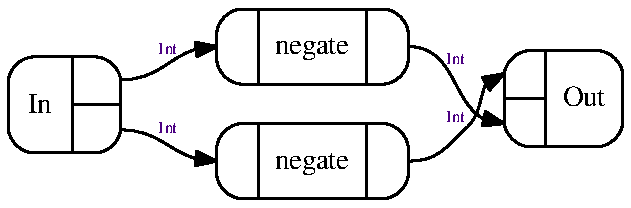
\includegraphics{neg-iv.pdf}
\end{frame}

\begin{frame}[fragile]{Addition}
  \begin{lstlisting}[frame=single]
  instance (Iv a ~ (a :* a), Num a, Ord a) => NumCat IF a where
    ..
    addC = pack (\ ((al,ah),(bl,bh)) -> (al+bl,ah+bh))
    ..
    {-# INLINE addC #-}
    ..
  \end{lstlisting}
\end{frame}

\begin{frame}[fragile]{Addition}
  \begin{lstlisting}[frame=single]
    runSynME "add" $ toCcc $ ivFun $ uncurry ((+) @Int)
  \end{lstlisting}
  \begin{lstlisting}[frame=single]
     uncurry (curry (apply . (exl &&& exr))) .
     (curry
      (
       (add . (exl . exl &&& exl . exr)
        &&&
        add . (exr . exl &&& exr . exr)
       ) . exr
      ) &&& id
     )
  \end{lstlisting}
\end{frame}

\begin{frame}[fragile]{Addition}
  \begin{lstlisting}[frame=single]
    runSynCirc "add" $ toCcc $ ivFun $ uncurry ((+) @Int)
  \end{lstlisting}
  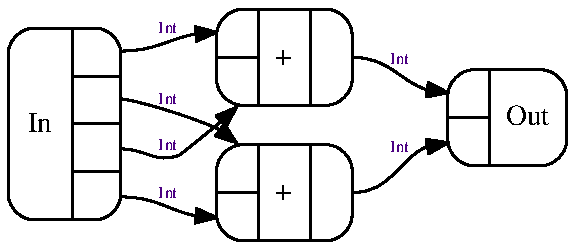
\includegraphics{add-iv.pdf}
\end{frame}

\begin{frame}[fragile]{Subtraction}
  \begin{lstlisting}[frame=single]
  instance (Iv a ~ (a :* a), Num a, Ord a) => NumCat IF a where
    ..
    subC = addC . second negateC
    ..
    {-# INLINE subC #-}
    ..
  \end{lstlisting}
  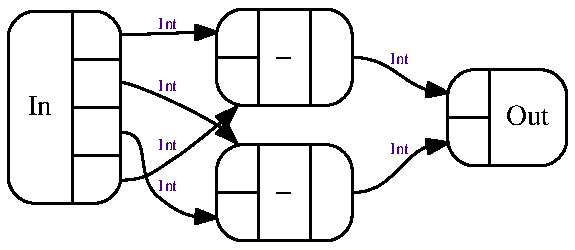
\includegraphics{sub-iv.pdf}
\end{frame}

\begin{frame}[fragile]{Multiplication}
  \begin{lstlisting}[frame=single]
  instance (Iv a ~ (a :* a), Num a, Ord a) => NumCat IF a where
    mulC = pack (\ ((al,ah),(bl,bh)) ->
               let cs = ((al*bl,al*bh),(ah*bl,ah*bh)) in
                 (min4 cs, max4 cs))
    ..
    {-# INLINE mulC #-}
  \end{lstlisting}
  \begin{center}
    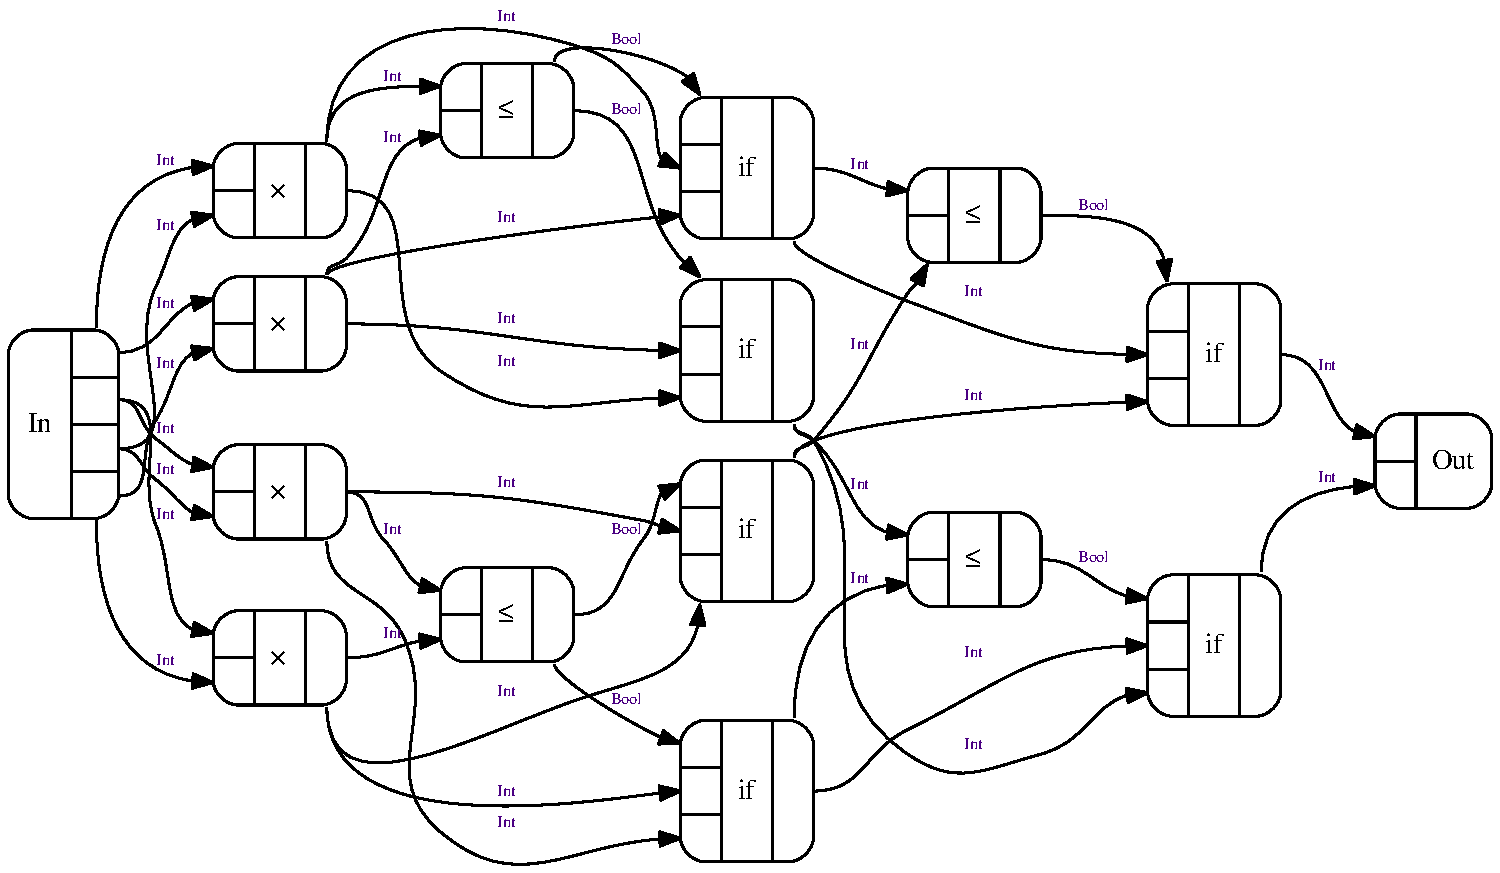
\includegraphics[width=0.8\textwidth]{mul-iv.pdf}
  \end{center}
\end{frame}

\begin{frame}[fragile]{Thrice}
  \begin{lstlisting}[frame=single]
     runSynCirc "thrice-iv" $ toCcc $ ivFun $ \ x -> 3 * x :: Int
  \end{lstlisting}
  \begin{center}
    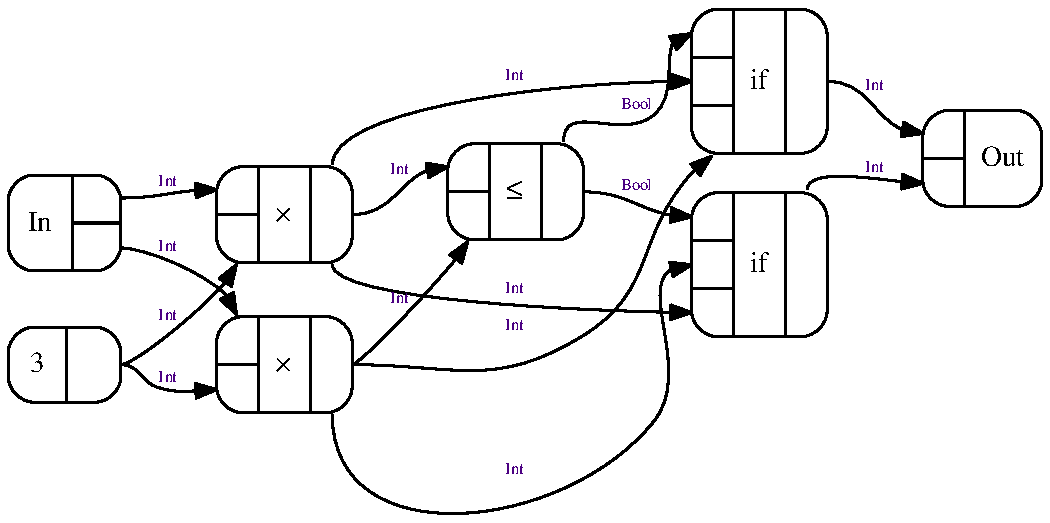
\includegraphics[width=0.8\textwidth]{thrice-iv.pdf}
  \end{center}
\end{frame}

\begin{frame}[fragile]{Square}
  \begin{lstlisting}[frame=single]
    runSynCirc "sqr-iv"    $ toCcc $ ivFun $ sqr @Int
  \end{lstlisting}
  \begin{center}
    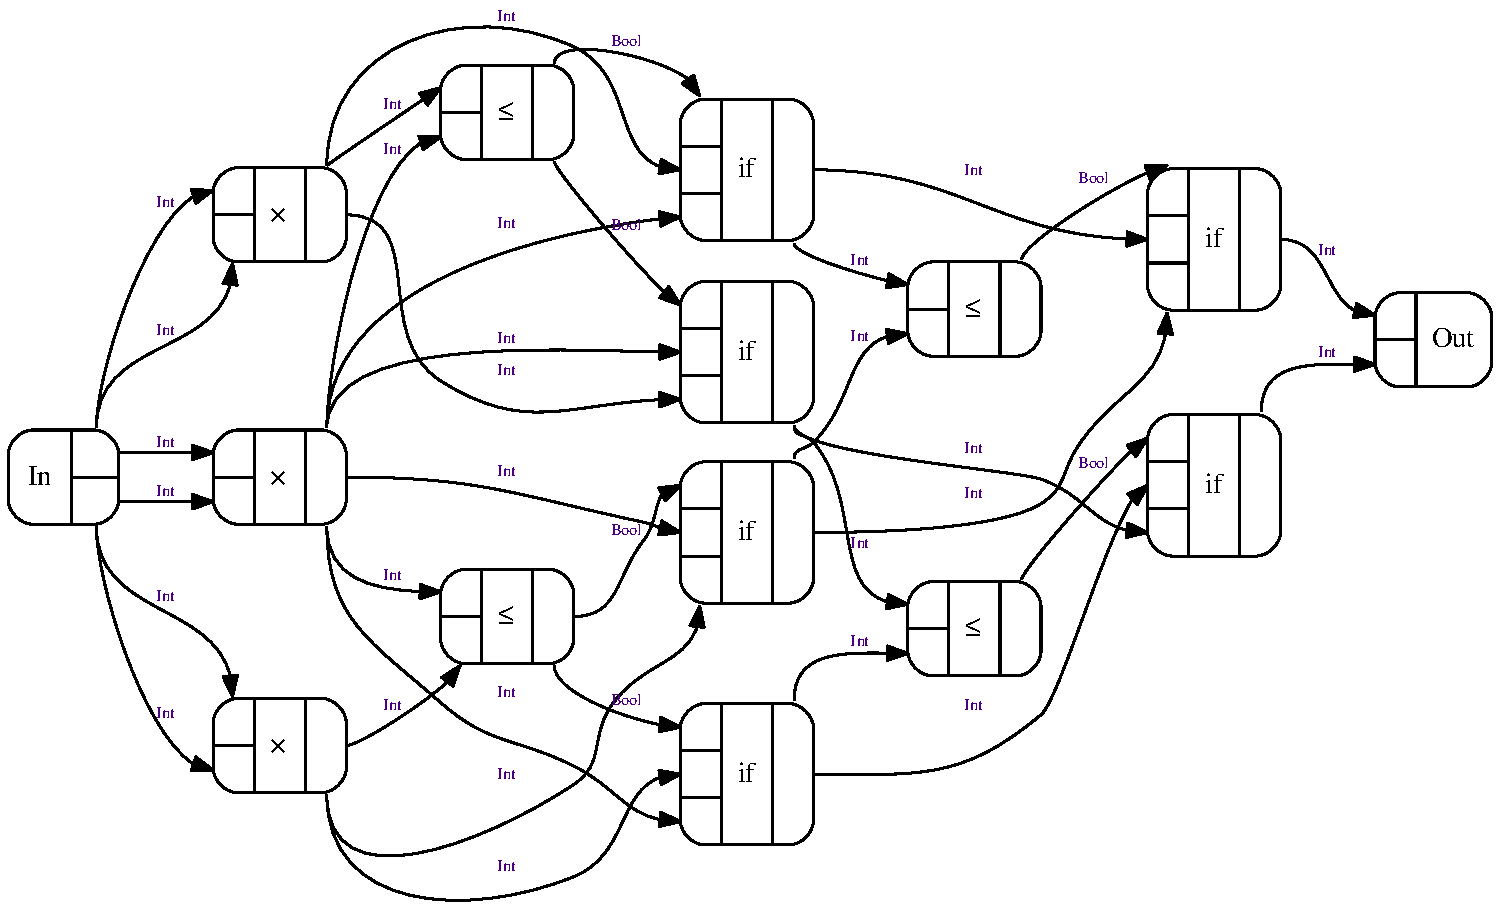
\includegraphics[width=1.0\textwidth]{sqr-iv.pdf}
  \end{center}
\end{frame}

\begin{frame}[fragile]{Magic Square}
  \begin{lstlisting}[frame=single]
    runSynCirc "magSqr-iv" $ toCcc $ ivFun $ magSqr @Int
  \end{lstlisting}
  \begin{center}
    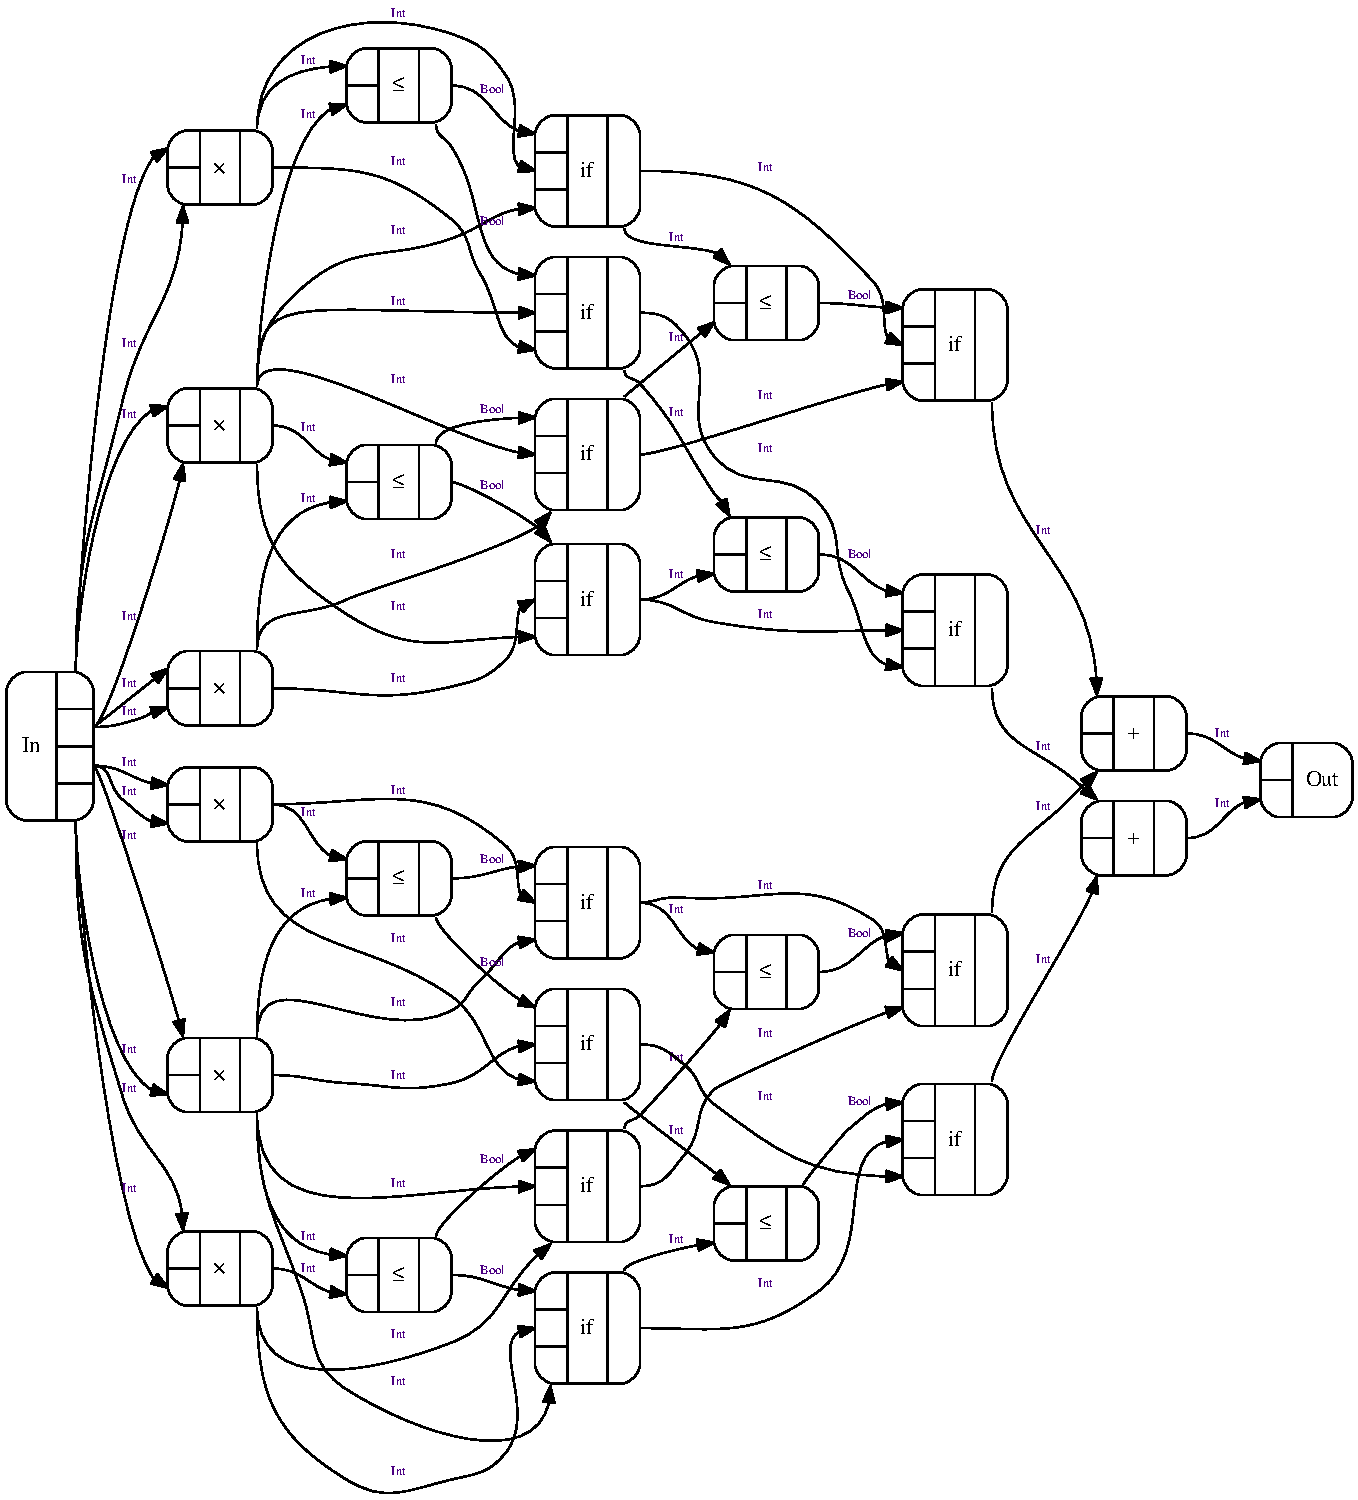
\includegraphics[width=0.5\textwidth]{magSqr-iv.pdf}
  \end{center}
\end{frame}

\section{Example: Category Products} %% Mark

\section{} %% Siva - Linear maps, derivatives; mention translation to hardware

\section{Future Work} %% Mark

\begin{frame}[fragile]{}
\end{frame}

\begin{frame}[fragile]{}
\end{frame}

\begin{frame}[fragile]{}
\end{frame}

\begin{frame}[fragile]{}
\end{frame}

\section{Conclusions} %% Mark

\section{Further Reading}

\begin{frame}[fragile]{Further Reading}

  \nocite{elkins_calculating_2009}
  \nocite{diel:blog}
  \nocite{milewski2014}

  \bibliography{ConCat-talk-20171115}
  \bibliographystyle{abbrv}

\end{frame}

\end{document}
